% LaTeX source for ``Python for Informatics: Exploring Information''
% Copyright (c)  2010-  Charles R. Severance, All Rights Reserved

\chapter{Arquivos}
%\chapter{Files}

\index{arquivo}
\index{tipo!arquivo}
%\index{file}
%\index{type!file}

\section{Persistência}
%\section{Persistence}

\index{persistência}
\index{memória secundária}
%\index{persistence}
%\index{secondary memory}

Até agora, aprendemos como escrever programas e comunicar nossas
intenções para a {\bf Unidade de Processamento Central} usando execução
condicional, funções e iterações. Aprendemos também como criar e usar 
estruturas de dados na {\bf Memória Principal}. A CPU e a memória é onde
nosso software executa. É o lugar onde todo ``o pensamento'' acontece.
%So far, we have learned how to write programs and communicate 
%our intentions to the {\bf Central Processing Unit} using conditional
%execution, functions, and iterations.  We have learned how to 
%create and use data structures in the {\bf Main Memory}.  The CPU 
%and memory are where our software works and runs.  It is where 
%all of the ``thinking'' happens.  

Mas se você se recordar das nossas discussões sobre arquitetura de hardware,
uma vez que a energia for desligada, tudo que estiver armazenado na CPU
ou na memória principal será apagado. Até agora, nossos
programas tem sido breves exercícios para aprender Python.
%But if you recall from our hardware architecture discussions,
%once the power is turned off, anything stored in either
%the CPU or main memory is erased.  So up to now, our
%programs have just been transient fun exercises to learn Python.

\beforefig
\centerline{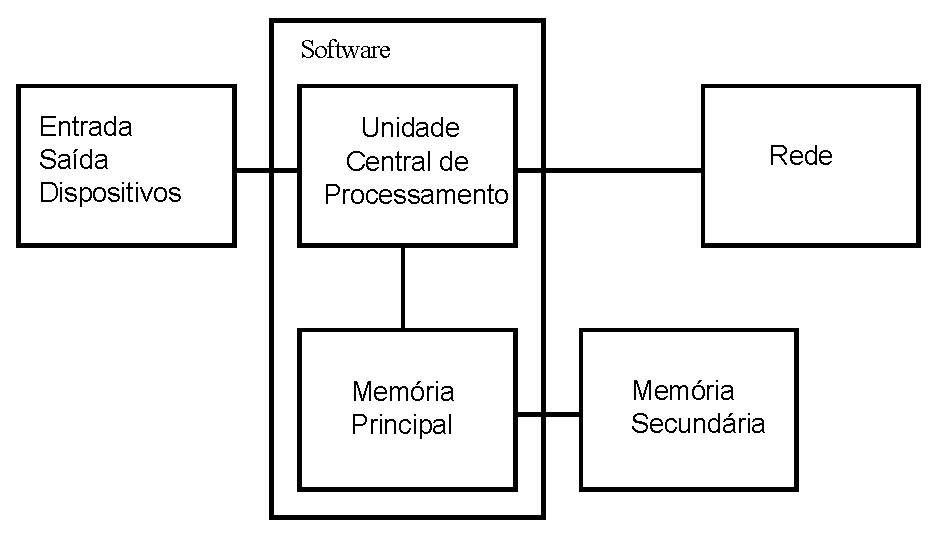
\includegraphics[height=2.50in]{figs2/arch3.eps}}
\afterfig
%\beforefig
%\centerline{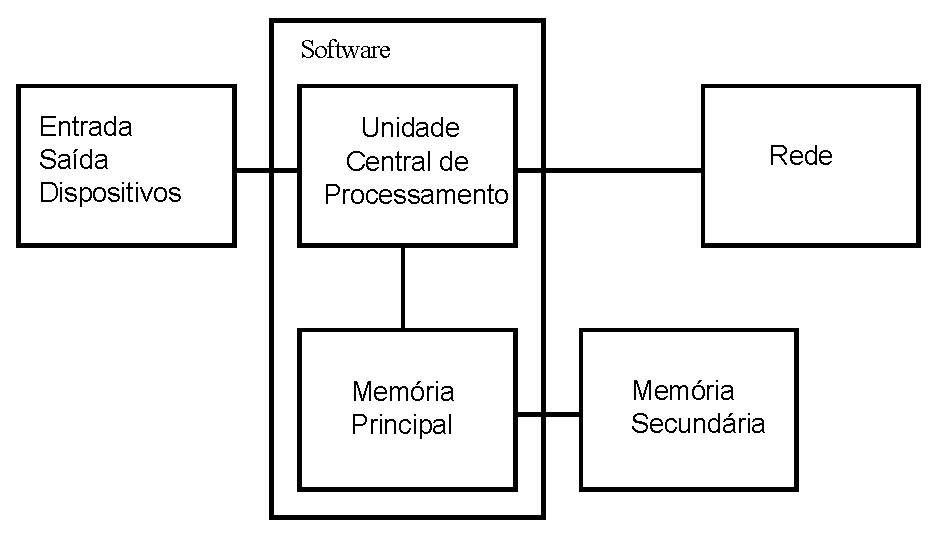
\includegraphics[height=2.50in]{figs2/arch3.eps}}
%\afterfig

Neste capítulo, começaremos a trabalhar com {\bf Memória Secundária}
(ou arquivos).
A memória secundária não é apagada quando a energia é desligada.
Ou no caso de um pen drive USB, o
dado que nós escrevemos a partir de nossos programas, pode ser
removido e transportado para outro sistema.
%In this chapter, we start to work with {\bf Secondary Memory} 
%(or files).
%Secondary memory is not erased even when the power is turned off.  
%Or in the case of a USB flash drive, the
%data we write from our programs can be removed from the 
%system and transported to another system.

Nós focaremos primeiramente na leitura e escrita de arquivos texto
tais como aqueles que criamos em um editor de texto. Depois iremos
trabalhar com arquivos de banco de dados que são arquivos binários,
especificamente desenhados para serem lidos e escritos através do nosso
software de banco de dados.
%We will primarily focus on reading and writing text files such as 
%those we create in a text editor.  Later we will see how to work
%with database files which are binary files, specifically designed to be read
%and written through database software.

\section{Lendo arquivos}
\index{arquivo!leitura}
\index{função open}
\index{função!open}
%\section{Opening files}
%\index{file!open}
%\index{open function}
%\index{function!open}

Quando queremos ler ou gravar um arquivo (nosso disco rígido, por exemplo),
devemos sempre abrir o arquivo primeiro através do comando {\bf open}. Abrir um
arquivo é uma comunicação com o seu sistema operacional, que sabe onde o dado
para cada arquivo é armazenado. Quando você abre um arquivo, você está pedindo
ao sistema operacional para encontrar o arquivo pelo nome e certificar-se de que
ele existe. Neste exemplo, abrimos o arquivo {\tt mbox.txt}, o qual deve ser armazenado
no mesmo diretório onde o seu programa Python está executando.
Você pode fazer o download deste arquivo a partir de:
\url{www.py4inf.com/code/mbox.txt}
%When we want to read or write a file (say on your hard drive), we first
%must {\bf open} the file.  Opening the file communicates with your operating
%system, which knows where the data for each file is stored.  When you open
%a file, you are asking the operating system to find the file by name
%and make sure the file exists.  In this example, we open the file 
%{\tt mbox.txt}, which should be stored in the same folder that you
%are in when you start Python.
%You can download this file from 
%\url{www.py4inf.com/code/mbox.txt}

\beforeverb
\begin{verbatim}
>>> fhand = open('mbox.txt')
>>> print fhand
<open file 'mbox.txt', mode 'r' at 0x1005088b0>
\end{verbatim}
\afterverb
%\beforeverb
%\begin{verbatim}
%>>> fhand = open('mbox.txt')
%>>> print fhand
%<open file 'mbox.txt', mode 'r' at 0x1005088b0>
%\end{verbatim}
%\afterverb
%

\index{manipulação de arquivo}
%\index{file handle}

Se o comando {\tt open} rodar com sucesso, o sistema operacional nos
retorna um {\bf manipulador de arquivo}. Este manipulador não contém
os dados do arquivo, mas apenas o ``ponteiro'' que nós podemos usar
para ler um dado. Você recebe um ponteiro se o arquivo requisitado
existir e se você tiver permissão para lê-lo.
%If the {\tt open} is successful, the operating system returns us a 
%{\bf file handle}.  The file handle is not the actual data contained
%in the file, but instead it is a ``handle'' that we can use to 
%read the data.   You are given a handle if the requested file
%exists and you have the proper permissions to read the file.

\beforefig
\centerline{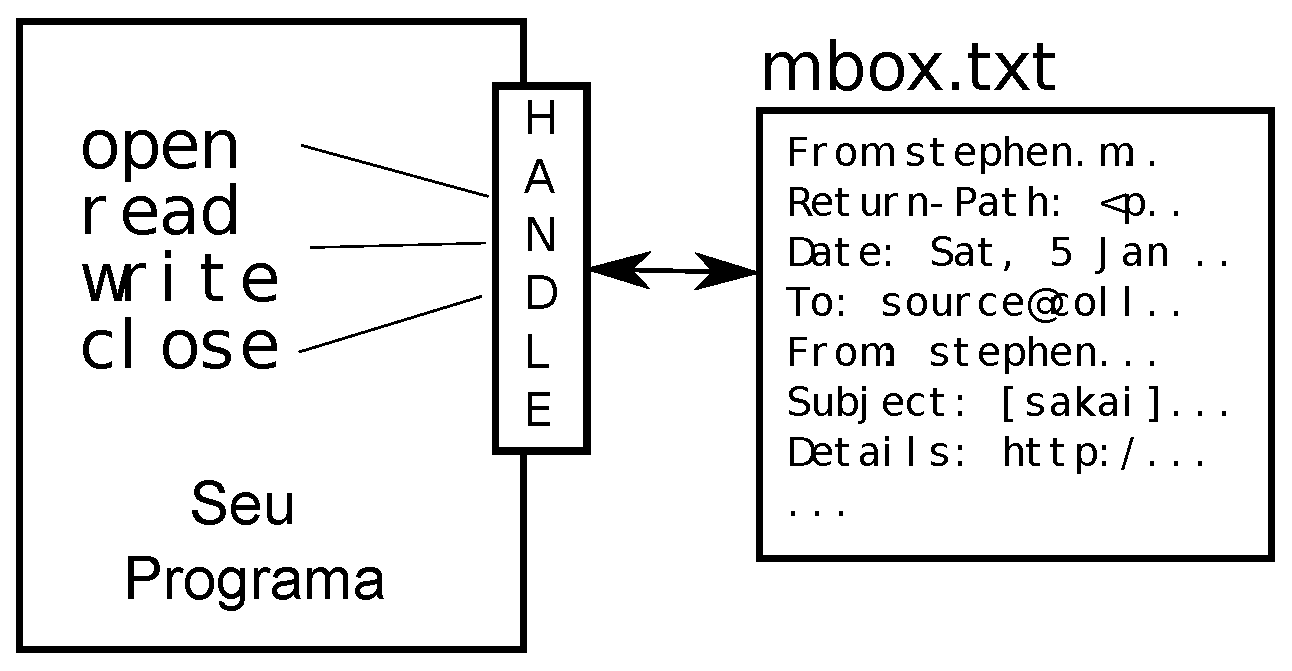
\includegraphics[height=1.75in]{figs2/handle.eps}}
\afterfig
%\beforefig
%\centerline{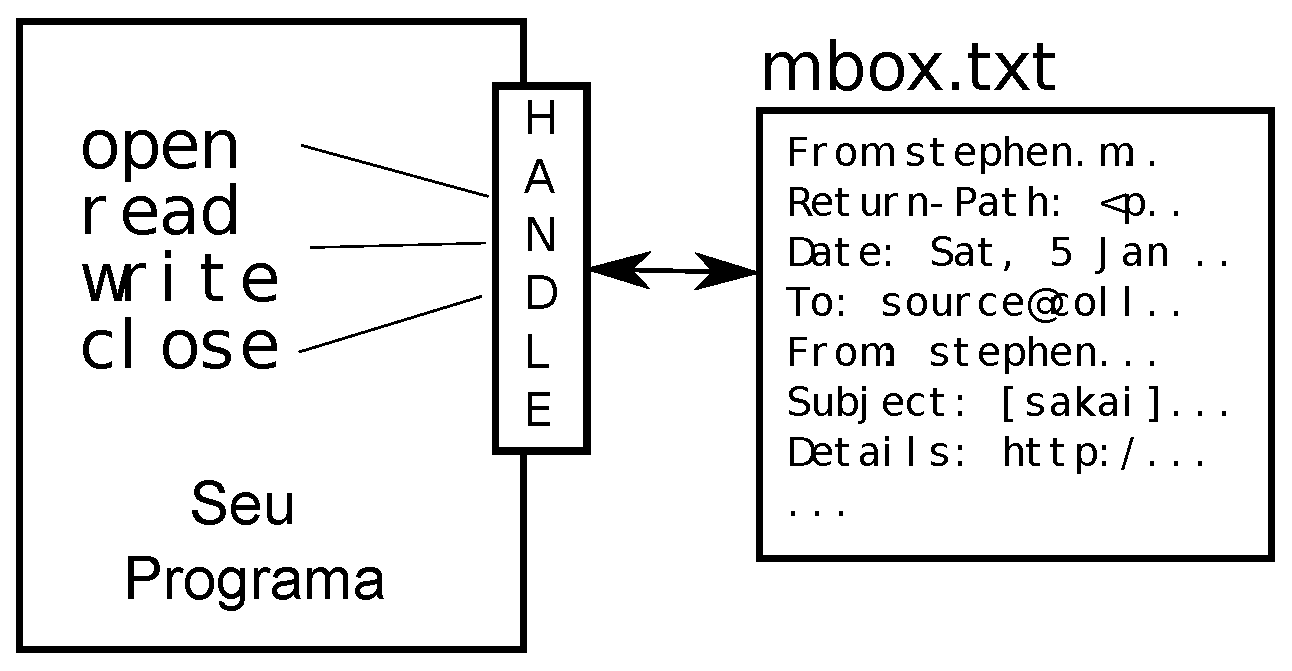
\includegraphics[height=1.75in]{figs2/handle.eps}}
%\afterfig

Se o arquivo não existir, {\tt open} ocorrerá um erro com a pilha de execução (traceback)
e você não conseguirá obter um ponteiro (handle) para acessar o conteúdo do arquivo: 
%If the file does not exist, {\tt open} will fail with a traceback and you 
%will not get a handle to access the contents of the file:

\beforeverb
\begin{verbatim}
>>> fhand = open('stuff.txt')
Traceback (most recent call last):
  File "<stdin>", line 1, in <module>
IOError: [Errno 2] No such file or directory: 'stuff.txt'
\end{verbatim}
\afterverb
%\beforeverb
%\begin{verbatim}
%>>> fhand = open('stuff.txt')
%Traceback (most recent call last):
%  File "<stdin>", line 1, in <module>
%IOError: [Errno 2] No such file or directory: 'stuff.txt'
%\end{verbatim}
%\afterverb

Mais tarde, vamos aprender a utilizar {\tt try} e {\tt except} para lidar 
com a situação onde tentamos abrir um arquivo que não existe.
%Later we will use {\tt try} and {\tt except} to deal more gracefully
%with the situation where we attempt to open a file that does 
%not exist.

\section{Arquivos texto e linhas}
%\section{Text files and lines}

Podemos imaginar um arquivo texto como um sequência de linhas, assim
como uma string em Python é uma sequência de caracteres. Por exemplo, esta
é um exemplo de um arquivo texto com registros de atividade de e-mail de várias
pessoas em um time de desenvolvimento em um projeto open source:
%A text file can be thought of as a sequence of lines, much like a Python
%string can be thought of as a sequence of characters.  For example, this
%is a sample of a text file which records mail activity from various
%individuals in an open source project development team:

\beforeverb
\begin{alltt}
From stephen.marquard@uct.ac.za Sat Jan  5 09:14:16 2008
Return-Path: <postmaster@collab.sakaiproject.org>
Date: Sat, 5 Jan 2008 09:12:18 -0500
To: source@collab.sakaiproject.org
From: stephen.marquard@uct.ac.za
Subject: [sakai] svn commit: r39772 - content/branches/
Details: http://source.sakaiproject.org/viewsvn/?view=rev\&rev=39772
...
\end{alltt}
\afterverb

O arquivo completo de iterações por e-mail está disponível em:
\url{www.py4inf.com/code/mbox.txt} 
e uma versão reduzida do arquivo está disponível em:
\url{www.py4inf.com/code/mbox-short.txt}.
Estes arquivos estão em um formato padrão de um arquivo contendo
múltiplas mensagens de e-mail. A expressão ``From '' separa as mensagens
e as linhas que começam com ``From:'' são parte da mensagem.
Para maiores informações sobre o formato mbox, veja:
\url{en.wikipedia.org/wiki/Mbox}. 
%The entire file of mail interactions is available from 
%\url{www.py4inf.com/code/mbox.txt} 
%and a shortened version of the file is available from
%\url{www.py4inf.com/code/mbox-short.txt}.
%These files are in a standard format for a file containing 
%multiple mail messages. The lines which start with 
%``From '' separate the messages and the lines which start 
%with ``From:'' are part of the messages. 
%For more information about the mbox format, see 
%\url{en.wikipedia.org/wiki/Mbox}. 

Para separar o arquivo em linhas, existe um caractere especial que
representa o ``fim da linha'' chamado de {\bf newline} caractere.
%To break the file into lines, there is a special character that 
%represents the ``end of the line'' called the {\bf newline} character.

\index{newline}
%\index{newline}

Em Python, representamos o caractere {\bf newline} como a string \textbackslash n,
uma constante string. Mesmo que essa expressão pareça ser dois caracteres, ela
é na verdade apenas um caractere simples. Quando imprimimos o valor da variável
``stuff'' no interpretador, ele nos mostra o \verb"\n" na string,
mas quando usamos {\tt print} para exibir, nós vemos uma string quebrada
em duas linhas pelo caractere newline.
%In Python, we represent the {\bf newline} character as a backslash-n in 
%string constants.  Even though this looks like two characters, it
%is actually a single character.  When we look at the variable by entering
%``stuff'' in the interpreter, it shows us the \verb"\n" in the string, 
%but when we use {\tt print} to show the string, we see the string broken
%into two lines by the newline character.

\beforeverb
\begin{verbatim}
>>> stuff = 'Hello\nWorld!'
>>> stuff
'Hello\nWorld!'
>>> print stuff
Hello
World!
>>> stuff = 'X\nY'
>>> print stuff
X
Y
>>> len(stuff)
3
\end{verbatim}
\afterverb

Você também pode ver que o tamanho da string \verb"'X\nY'" é \emph{três [three]}
caracteres porque o caractere newline é um único caractere simples.
%You can also see that the length of the string \verb"'X\nY'" is \emph{three}
%characters because the newline character is a single character.

Então, quando olhamos as linhas em um arquivo, nós precisamos \emph{imaginar}
que ele é uma espécie de caractere invisível que faz com que o fim de cada linha
seja de fato, o fim da linha.
%So when we look at the lines in a file, we need to \emph{imagine}
%that there is a special invisible character called the newline at
%the end of each line that marks the end of the line.  

 \beforeverb
 \begin{alltt}
 From stephen.marquard@uct.ac.za Sat Jan  5 09:14:16 2008\verb"\n"\\
 Return-Path: <postmaster@collab.sakaiproject.org>\verb"\n"\\
 Date: Sat, 5 Jan 2008 09:12:18 -0500\verb"\n"\\
 To: source@collab.sakaiproject.org\verb"\n"\\
 From: stephen.marquard@uct.ac.za\verb"\n"\\
 Subject: [sakai] svn commit: r39772 - content/branches/\verb"\n"\\
 Details: http://source.sakaiproject.org/viewsvn/?view=rev\&rev=39772\verb"\n"\\
 ...
 \end{alltt}
 \afterverb

Observe que o caractere newline separa os caracteres
no arquivo em linhas.
%So the newline character separates the characters 
%in the file into lines.

\section{Lendo arquivos}
%\section{Reading files}

\index{arquivo!leitura}
\index{contador}
%\index{file!reading}
%\index{counter}

O {\bf ponteiro para o arquivo} não contém o dado do arquivo,
é muito fácil construir um laço {\tt for} para ler o arquivo inteiro
e contar quantas linhas existem.
%While the {\bf file handle} does not contain the data for the file,
%it is quite easy to construct a {\tt for} loop to read through 
%and count each of the lines in a file:

\beforeverb
\begin{verbatim}
fhand = open('mbox.txt')
count = 0
for line in fhand:
    count = count + 1
print 'Line Count:', count

python open.py 
Line Count: 132045
\end{verbatim}
\afterverb

Nós podemos utilizar o ponteiro do arquivo como uma sequência no nosso
loop {\tt for}. Nosso loop {\tt for} conta o número de linhas no
arquivo e então imprime. Uma tradução grotesca do loop {\tt for} para
o português seria, ``para cada linha do arquivo representada pelo ponteiro
do arquivo, adicione um à variável {\tt count}.''
%We can use the file handle as the sequence in our {\tt for} loop.  
%Our {\tt for} loop simply counts the number of lines in the 
%file and prints them out.  The rough translation of the {\tt for}
%loop into English is, ``for each line in the file represented by the file
%handle, add one to the {\tt count} variable.''

A razão pela qual a função {\tt open} não lê o arquivo inteiro é que
o arquivo pode ser muito grande com vários gigabytes de dados.
A instrução {\tt open} recebe a mesma quantidade de tempo sem levar em
consideração o tamanho do arquivo.
%The reason that the {\tt open} function does not read the entire file
%is that the file might be quite large with many gigabytes of data.
%The {\tt open} statement takes the same amount of time regardless of the
%size of the file.  The {\tt for} loop actually causes the data to be 
%read from the file.

Quando um arquivo é lido usando um laço {\tt for} desta maneira, o Python
divide o dado do arquivo em linhas separadas pelo caractere newline.
O Python lê cada linha até encontrar o newline e então inclui o newline
como o último caractere da variável {\tt line} para cada iteração do 
laço {\tt for}. 
%When the file is read using a {\tt for} loop in this manner, Python
%takes care of splitting the data in the file into separate lines using
%the newline character.  Python reads each line through 
%the newline and includes
%the newline as the last character in the {\tt line} variable for each 
%iteration of the {\tt for} loop.

Pelo fato de o laço {\tt for} ler o dado uma linha de cada vez, ele
consegue eficientemente ler e contar as linhas em um arquivos grandes
sem estourar a memória do computador para armazenar os dados. O programa
acima pode contar as linhas em qualquer tamanho de arquivo usando pouca
quantidade de memória uma vez que cada linha é lida, contada e então
descartada. 
%Because the {\tt for} loop reads the data one line at a time, it can efficiently
%read and count the lines in very large files without running 
%out of main memory to store the data.  The above program can 
%count the lines in any size file using very little memory since 
%each line is read, counted, and then discarded.

Se você souber que o arquivo é relativamente pequeno comparado ao 
tamanho total da memória principal, você pode ler o arquivo inteiro
para uma única string usando o método {\tt read} no ponteiro do arquivo
{\tt handle}.
%If you know the file is relatively small compared to the size of 
%your main memory, you can read the whole file into one string
%using the {\tt read} method on the file handle.

\beforeverb
\begin{verbatim}
>>> fhand = open('mbox-short.txt')
>>> inp = fhand.read()
>>> print len(inp)
94626
>>> print inp[:20]
From stephen.marquar
\end{verbatim}
\afterverb

Neste exemplo, o conteúdo total (todos os 94.626 caracteres)
do arquivo {\tt mbox-short.txt} são lidos diretamente para a
variável {\tt inp}. Nós usamos o método de fatiar a string {\tt slice}
para imprimir os primeiros 20 caracteres dos dados armazenados na string
{\tt inp}.
%In this example, the entire contents (all 94,626 characters) 
%of the file {\tt mbox-short.txt} are read directly into the 
%variable {\tt inp}.  We use string slicing to print out the first
%20 characters of the string data stored in {\tt inp}.

Quando o arquivo é lido deste modo, todos os caracteres incluindo 
todas as linhas e caracteres newline são uma única e grande string
dentro da variável {\bf inp}.
Lembre que este modo de utilizar a função {\tt open} deve somente ser
usado se o tamanho do arquivo lido couber perfeitamente na memória 
principal do seu computador.
%When the file is read in this manner, all the characters including 
%all of the lines and newline characters are one big string 
%in the variable {\bf inp}.  
%Remember that this form of the {\tt open} function should only be used
%if the file data will fit comfortably in the main memory 
%of your computer.

Se o arquivo for muito grande para a memória principal, você deve
escrever seu programa para ler o arquivo em blocos, usando um laço 
{\tt for} ou {\tt while}.
%If the file is too large to fit in main memory, you should write
%your program to read the file in chunks using a {\tt for} or {\tt while}
%loop.

\section{Fazendo buscas em um arquivo}
%\section{Searching through a file}

Quando você estiver procurando algo dentro de um arquivo, esta
é uma forma comum de se percorrer todo o arquivo, ignorando a 
maioria das linhas e somente processando aquelas que atendam a uma
condição particular. Nós podemos combinar padrões para leitura em
um arquivo com os métodos da classe string para construir mecanismos 
simples de busca.
%When you are searching through data in a file, it
%is a very common pattern to read through a file, ignoring most
%of the lines and only processing lines which meet a particular condition.
%We can combine the pattern for reading a file with string methods
%to build simple search mechanisms.

\index{padrão de filtro}
\index{padrão!filtro}
%\index{filter pattern}
%\index{pattern!filter}

Por exemplo, se quisermos ler o arquivo, imprimindo apenas as linhas
que iniciarem com o prefixo ``From:'', podemos usar o método da classe 
string {\bf startswith} para selecionar apenas as linhas com o prefixo 
desejado:
%For example, if we wanted to read a file and only print out lines
%which started with the prefix ``From:'', we could use the 
%string method {\bf startswith} to select only those lines with
%the desired prefix:

\beforeverb
\begin{verbatim}
fhand = open('mbox-short.txt')
for line in fhand:
    if line.startswith('From:') :
        print line
\end{verbatim}
\afterverb

Quando este programa executa, obtemos a seguinte saída:
%When this program runs, we get the following output:

\beforeverb
\begin{verbatim}
From: stephen.marquard@uct.ac.za

From: louis@media.berkeley.edu

From: zqian@umich.edu

From: rjlowe@iupui.edu
...
\end{verbatim}
\afterverb

O programa funcionou, uma vez que a saída imprimiu apenas aquelas
linhas que iniciam com o prefixo ``From:''. Mas porque iríamos querer
as linhas em branco? Isto se deve ao caractere invisível {\bf newline}.
Cada uma das linhas terminam com um newline, então a instrução {\tt print}
imprime a string contida na variável {\bf line} o que inclui um newline
e então a instrução {\t print} adiciona \emph{outro} newline, resultando
no efeito de duplo espaço que pudemos visualizar.
%The output looks great since the only lines we are seeing are those 
%which start with ``From:'', but why are we seeing the extra blank
%lines?  This is due to that invisible {\bf newline} character.
%Each of the lines ends with a newline, so the {\tt print} 
%statement prints the string in the variable {\bf line} which includes
%a newline and then {\tt print} adds \emph{another} newline, resulting
%in the double spacing effect we see.

Nós podemos utilizar o método slicing para imprimir todos os caracteres
menos o último, mas um método mais interessante é utilizar o método 
{\bf strip} para remover o espaço em branco do lado direito da string,
como segue:
%We could use line slicing to print all but the last character, but 
%a simpler approach is to use the {\bf rstrip} method which strips
%whitespace from the right side of a string as follows:

\beforeverb
\begin{verbatim}
fhand = open('mbox-short.txt')
for line in fhand:
    line = line.rstrip()
    if line.startswith('From:') :
        print line
\end{verbatim}
\afterverb

Quando este programa executa, obtemos a seguinte saída:
%When this program runs, we get the following output:

\beforeverb
\begin{verbatim}
From: stephen.marquard@uct.ac.za
From: louis@media.berkeley.edu
From: zqian@umich.edu
From: rjlowe@iupui.edu
From: zqian@umich.edu
From: rjlowe@iupui.edu
From: cwen@iupui.edu
...
\end{verbatim}
\afterverb

Conforme seus programas de processamento de arquivo se tornam mais 
complicados, você pode estruturar seus laços com a instrução 
{\tt continue}. A ideia básica do laço de busca é que você procura
por linhas ``interessantes'' e efetivamente pula aquelas ``não interessantes''.
E então quando encontrarmos uma linha interessante, podemos fazer algo com ela.
%As your file processing programs get more complicated, you may want 
%to structure your search loops using {\tt continue}.  The basic idea 
%of the search loop is that you are looking for ``interesting'' lines
%and effectively skipping ``uninteresting'' lines.  And then when we
%find an interesting line, we do something with that line.

Podemos estruturar o laço para seguir o padrão de
pular linhas que não interessam, como segue:
%We can structure the loop to follow the
%pattern of skipping uninteresting lines as follows:

\beforeverb
\begin{verbatim}
fhand = open('mbox-short.txt')
for line in fhand:
    line = line.rstrip()
    # Skip 'uninteresting lines'
    if not line.startswith('From:') :
        continue
    # Process our 'interesting' line
    print line
\end{verbatim}
\afterverb

A saída do programa é a mesma. As linhas que não são
interessantes são aquelas que não começam com ``From:'',
as quais nós pulamos através da instrução {\tt continue}.
As linhas interessantes (i.e., aquelas que começam com ``From:'')
são processadas pelo nosso programa.
%The output of the program is the same.  In English, the 
%uninteresting lines are those which do not start 
%with ``From:'', which we skip using {\tt continue}.
%For the ``interesting'' lines (i.e., those that start with ``From:'')
%we perform the processing on those lines.

Podemos usar o método da classe string {\tt find}, para simular
uma busca de um editor de texto que procura por uma string em todas
as linhas de um arquivo onde ela aparecer, não importa a posição da
linha. A instrução {\tt find} procura pela ocorrência de uma string 
em outra, retornando o índice da posição encontrada ou -1 caso não 
encontre. Podemos escrever o seguinte laço para mostrar as linhas que
contém a string ``@uct.ac.za'' (i.e. originadas na Universidade de
Cape Town na África do Sul):
%We can use the {\tt find} string method to simulate a text editor
%search that finds lines where the search string is anywhere in the line.  
%Since {\tt find} looks for an occurrence of a string within another
%string and either returns the position of the string or -1 if the string
%was not found, we can write the following loop to show lines which
%contain the string ``@uct.ac.za'' (i.e., they come from the University 
%of Cape Town in South Africa):

\beforeverb
\begin{verbatim}
fhand = open('mbox-short.txt')
for line in fhand:
    line = line.rstrip()
    if line.find('@uct.ac.za') == -1 : 
        continue
    print line
\end{verbatim}
\afterverb

Que produz a seguinte saída:
%Which produces the following output:

\beforeverb
\begin{verbatim}
From stephen.marquard@uct.ac.za Sat Jan  5 09:14:16 2008
X-Authentication-Warning: set sender to stephen.marquard@uct.ac.za using -f
From: stephen.marquard@uct.ac.za
Author: stephen.marquard@uct.ac.za
From david.horwitz@uct.ac.za Fri Jan  4 07:02:32 2008
X-Authentication-Warning: set sender to david.horwitz@uct.ac.za using -f
From: david.horwitz@uct.ac.za
Author: david.horwitz@uct.ac.za
...
\end{verbatim}
\afterverb

\section{Deixando o usuário escolher o nome do arquivo}
%\section{Letting the user choose the file name}

Nós não queremos ter que editar nosso código Python toda vez
que tivermos que processar um arquivo diferente. É melhor
pedir que o usuário digite o nome do arquivo cada vez que
o programa executar, assim nosso programa pode ser utilizado
para executar diferentes arquivos sem ter que ficar alterando
o script Python.
%We really do not want to have to edit our Python code
%every time we want to process a different file.  It would 
%be more usable to ask the user to enter the file name string 
%each time the program runs so they can use our 
%program on different files without changing the Python code.

Isto é muito fácil de se fazer, basta utilizarmos a instrução
\verb"raw_input" como mostrado a seguir:
%This is quite simple to do by reading the file name from
%the user using \verb"raw_input" as follows:

\beforeverb
\begin{verbatim}
fname = raw_input('Enter the file name: ')
fhand = open(fname)
count = 0
for line in fhand:
    if line.startswith('Subject:') :
        count = count + 1
print 'There were', count, 'subject lines in', fname
\end{verbatim}
\afterverb

O nome do arquivo é lido através da entrada do usuário e armazenado
em uma variável chamada {\tt fname} e então o arquivo é aberto. Desta
forma podemos executar o programa diversas vezes na leitura de 
diferentes arquivos.
%We read the file name from the user and place it in a variable
%named {\tt fname} and open that file.  Now we can run the program 
%repeatedly on different files.

\beforeverb
\begin{verbatim}
python search6.py 
Enter the file name: mbox.txt
There were 1797 subject lines in mbox.txt

python search6.py 
Enter the file name: mbox-short.txt
There were 27 subject lines in mbox-short.txt
\end{verbatim}
\afterverb

Antes de espiar a próxima seção, dê uma olhada no programa acima
e pergunte a você mesmo, ``O que pode dar errado aqui?'' ou ``O que
será que o nosso amigo usuário pode querer fazer que vá fazer com que
o nosso pequeno programa terminar com um erro inesperado e um traceback,
fazendo com que olhemos de uma forma não tão bacana para os olhos dos
nossos queridos usuários?''
%Before peeking at the next section, take a look at the above program
%and ask yourself, ``What could go possibly wrong here?'' or ``What might our
%friendly user do that would cause our nice little program to 
%ungracefully exit with a traceback, making us look not-so-cool 
%in the eyes of our users?''

\section{Usando {\tt try, except,} e {\tt open}}
%\section{Using {\tt try, except,} and {\tt open}}

Eu disse para você não espiar. Esta é a sua última chance
%I told you not to peek.  This is your last chance.

O que aconteceria se o usuário digitasse qualquer outra coisa
que não fosse o nome de um arquivo?
%What if our user types something that is not a file name?

\beforeverb
\begin{verbatim}
python search6.py 
Enter the file name: missing.txt
Traceback (most recent call last):
  File "search6.py", line 2, in <module>
    fhand = open(fname)
IOError: [Errno 2] No such file or directory: 'missing.txt'

python search6.py 
Enter the file name: na na boo boo
Traceback (most recent call last):
  File "search6.py", line 2, in <module>
    fhand = open(fname)
IOError: [Errno 2] No such file or directory: 'na na boo boo'
\end{verbatim}
\afterverb

Não dê risada, os usuários tentarão de todas as formas fazer com que
o nosso programa dê erros---seja com um propósito ou com intenção
maliciosa. Na verdade, uma importante atividade de qualquer time de 
desenvolvimento de software é uma pessoa ou grupo chamado {Quality Assurance}
(ou QA), cuja principal responsabilidade é fazer as coisas mais loucas
possíveis na tentativa de quebrar o software que o programador criou.
%Do not laugh, users will eventually do every possible thing they can do 
%to break your programs---either on purpose or with malicious intent.
%As a matter of fact, an important part of any software development
%team is a person or group called {\bf Quality Assurance} (or QA for short)
%whose very job it is to do the craziest things possible in an attempt
%to break the software that the programmer has created.

\index{Quality Assurance}
\index{QA}
%\index{Quality Assurance}
%\index{QA}

O time de QA é responsável por encontrar falhas em programas antes que
ele seja entregue aos usuários finais que estão pagando o software
ou o salário dos programadores. Então, o time QA são os melhores amigos
dos desenvolvedores.
%The QA team is responsible for finding the flaws in programs before 
%we have delivered the program to the end users who may be purchasing the
%software or paying our salary to write the software.  So the QA team
%is the programmer's best friend.

\index{instrução try}
\index{instrução!try}
\index{função open}
\index{função!open}
\index{exceção!IOError}
\index{IOError}
%\index{try statement}
%\index{statement!try}
%\index{open function}
%\index{function!open}
%\index{exception!IOError}
%\index{IOError}

Então, agora que encontramos uma falha no programa, podemos consertá-lo
usando a estrutura {\tt try}/{\tt except}. Podemos assumir que a chamada 
{\tt open} pode falhar e adicionar um código de tratamento para quando
o {\tt open} falhar, como segue:
%So now that we see the flaw in the program, we can elegantly fix it using
%the {\tt try}/{\tt except} structure.  We need to assume that the {\tt open}
%call might fail and add recovery code when the {\tt open} fails
%as follows:

\beforeverb
\begin{verbatim}
fname = raw_input('Enter the file name: ')
try:
    fhand = open(fname)
except:
    print 'File cannot be opened:', fname
    exit()

count = 0
for line in fhand:
    if line.startswith('Subject:') : 
        count = count + 1
print 'There were', count, 'subject lines in', fname
\end{verbatim}
\afterverb

A função {\tt exit} faz que com o programa termine. Esta é uma
função que chamamos e que nunca retorna. Agora quando nosso usuário
(ou o time QA) digitar nomes bobos ou ruins para o nome do arquivo,
nós ``capturamos'' os erros e tratamos de uma forma adequada.
%The {\tt exit} function terminates the program.  It is a function
%that we call that never returns.  Now when our user (or 
%QA team) types in silliness or bad file names, 
%we ``catch'' them and recover gracefully:

\beforeverb
\begin{verbatim}
python search7.py
Enter the file name: mbox.txt
There were 1797 subject lines in mbox.txt

python search7.py
Enter the file name: na na boo boo
File cannot be opened: na na boo boo
\end{verbatim}
\afterverb

\index{Pythônico}
%\index{Pythonic}

Proteger a chamada da função {\tt open} é um bom
exemplo do uso correto da instrução {\tt try} e 
{\tt catch} em um programa Python. Utilizamos o termo
``Pythônico'' quando estamos fazendo do ``jeito Python''.
Podemos dizer que o exemplo acima é o jeito Pythônico
de se abrir um arquivo.
%Protecting the {\tt open} call is a good example 
%of the proper use of {\tt try}
%and {\tt except} in a Python program.  We use the term
%``Pythonic'' when we are doing something the ``Python
%way''.  We might say that the above example is 
%the Pythonic way to open a file.

Quando você se tornar mais qualificado em Python, pode
ajudar outros programadores Python a decidir qual de duas
soluções equivalentes para um determinado problema é
``mais Pythônica''. O objetivo de ser ``mais Pythônico''
remete à noção de que programação é parte da engenharia
e da arte. Não estamos interessados em apenas fazer algo
funcionar, queremos que a nossa solução seja elegante
e apreciada por nossos colegas.
%Once you become more skilled in Python, you can engage
%in repartee with other Python programmers to decide
%which of two equivalent solutions to a problem is 
%``more Pythonic''.  The goal to be ``more Pythonic'' 
%captures the notion that programming is part engineering
%and part art.  We are not always interested
%in just making something work, we also want
%our solution to be elegant and to be appreciated as 
%elegant by our peers.

\section{Escrevendo arquivos}
%\section{Writing files}

\index{arquivos!escrita}
%\index{file!writing}

Para escrever um arquivo, você deve abri-lo no
modo \verb"'w'" como segundo parâmetro.
%To write a file, you have to open it with mode
%\verb"'w'" as a second parameter:

\beforeverb
\begin{verbatim}
>>> fout = open('output.txt', 'w')
>>> print fout
<open file 'output.txt', mode 'w' at 0xb7eb2410>
\end{verbatim}
\afterverb

Se o arquivo já existir, abri-lo no modo escrita irá limpar o
conteúdo do arquivo e iniciar uma escrita limpa, então tenha 
cuidado! Se o arquivo não existir, um novo será criado.
%If the file already exists, opening it in write mode clears out
%the old data and starts fresh, so be careful!
%If the file doesn't exist, a new one is created.

O método {\tt write} de um objeto tratador ``(handle)'' de 
arquivo colocará dados dentro dele.
%The {\tt write} method of the file handle object 
%puts data into the file.

\beforeverb
\begin{verbatim}
>>> line1 = "This here's the wattle,\n"
>>> fout.write(line1)
\end{verbatim}
\afterverb

\index{newline}
%\index{newline}

Novamente, o objeto file mantém o endereço de onde o arquivo 
está, assim, se você chamar {\tt write} novamente, irá adicionar
dados ao final do arquivo.
%Again, the file object keeps track of where it is, so if
%you call {\tt write} again, it adds the new data to the end.

Devemos nos certificar de gerenciar o fim das linhas conforme
escrevemos em um arquivo, explicitamente inserindo o caractere
newline quando quisermos finalizar a linha. A instrução {\tt print}
adiciona automaticamente uma nova linha. A instrução {\tt print}
automaticamente adiciona uma nova linha, mas o método {\tt write}
não adiciona automaticamente uma nova linha.
%We must make sure to manage the ends of lines as we write
%to the file by explicitly inserting the newline character
%when we want to end a line.  The {\tt print} statement 
%automatically appends a newline, but the {\tt write} 
%method does not add the newline automatically.

\beforeverb
\begin{verbatim}
>>> line2 = 'the emblem of our land.\n'
>>> fout.write(line2)
\end{verbatim}
\afterverb

Quando você terminar de escrever, terá que fechar o arquivo
para se certificar de que o último bit de dados será escrito
fisicamente para o disco, assim a informação não será perdida
quando a energia desligar. 
%When you are done writing, you have to close the file
%to make sure that the last bit of data is physically written
%to the disk so it will not be lost if the power goes off.

\beforeverb
\begin{verbatim}
>>> fout.close()
\end{verbatim}
\afterverb

Podemos fechar os arquivos que abrirmos para leitura também,
mas podemos ser um pouco negligentes somente se estivermos
abrindo alguns poucos arquivos desde que o Python se certifique
de fechar todos os arquivos que foram abertos quando o programa
finalizar. Quando escrevermos arquivos, temos que fechar explicitamente
usando a instrução {\tt close} para não corromper o arquivo. 
%We could close the files which we open for read as well, 
%but we can be a little sloppy if we are only opening a few
%files since Python makes sure that all open files are 
%closed when the program ends.  When we are writing files, 
%we want to explicitly close the files so as to leave nothing
%to chance.

\index{método close}
\index{método!close}
%\index{close method}
%\index{method!close}

\section{Depurando ou ``Debugando''}
%\section{Debugging}

\index{debugando}
\index{espaço em branco}
%\index{debugging}
%\index{whitespace}

Quando você estiver lendo e escrevendo arquivos, você pode ter 
problemas com espaços em branco. Estes erros podem ser difíceis 
de se depurar porque espaços, tabs e novas linhas são normalmente
invisíveis:
%When you are reading and writing files, you might run into problems
%with whitespace.  These errors can be hard to debug because spaces,
%tabs, and newlines are normally invisible:

\beforeverb
\begin{verbatim}
>>> s = '1 2\t 3\n 4'
>>> print s
1 2	 3
 4
\end{verbatim}
\afterverb
 
\index{função repr}
\index{função!repr}
\index{representação de uma string}
%\index{repr function}
%\index{function!repr}
%\index{string representation}

A função padrão {\tt repr} pode ajudar. Recebe qualquer objeto como um
argumento e retorna a representação da string de um objeto. Para strings,
os espaços em branco são representados como caracteres com sequências
de \textbackslash n:
%The built-in function {\tt repr} can help.  It takes any object as an
%argument and returns a string representation of the object.  For
%strings, it represents whitespace
%characters with backslash sequences:

\beforeverb
\begin{verbatim}
>>> print repr(s)
'1 2\t 3\n 4'
\end{verbatim}
\afterverb

Isto pode ser muito interessante para depuração.
%This can be helpful for debugging.

Um outro problema que você pode ter é que diferentes sistemas
usam diferentes caracteres para indicar o fim da linha. Alguns
sistemas usam o newline, representado por \verb"\n". Outros usam
um caractere de retorno, representado por \verb"\r". Alguns usam os
dois. Se você mover-se entre estes diferentes sistemas, algumas 
inconsistências podem causar problemas.
%One other problem you might run into is that different systems
%use different characters to indicate the end of a line.  Some
%systems use a newline, represented \verb"\n".  Others use
%a return character, represented \verb"\r".  Some use both.
%If you move files between different systems, these inconsistencies
%might cause problems.

\index{caractere fim de linha}
%\index{end of line character}

Para a maioria dos sistemas, existem aplicativos para converter
de um formato para o outro. Você pode achá-los (e ler mais sobre
este assunto) em \url{wikipedia.org/wiki/Newline}. Ou, naturalmente,
você pode escrever o seu próprio aplicativo.
%For most systems, there are applications to convert from one
%format to another.  You can find them (and read more about this
%issue) at \url{wikipedia.org/wiki/Newline}.  Or, of course, you
%could write one yourself.

%% TBD - Doesn't Python take care of this for us????

\section{Glossário}
%\section{Glossary}

\begin{description}

\item[catch:] Para prevenir uma exceção de terminar um programa
usando as instruções {\tt try} e {\tt except}.
\index{catch}
%\item[catch:] To prevent an exception from terminating
%a program using the {\tt try} and {\tt except} statements.
%\index{catch}

\item[newline:] Um caractere especial utilizado em arquivos e strings
para indicar o fim de uma linha.
\index{newline}
%\item[newline:] A special character used in files and strings to indicate
%the end of a line.
%\index{newline}

\item[Pythonic:] Uma técnica que funciona elegantemente no Python.
``Usar try e except é um jeito \emph{Pythônico} de se recuperar de 
arquivos não existentes, por exemplo''.
\index{Pythonic}
%\item[Pythonic:] A technique that works elegantly in Python.
%``Using try and except is the \emph{Pythonic} way to recover from 
%missing files''.
%\index{Pythonic}

\item[Controle da Qualidade - QA:] Uma pessoa ou time focado em 
garantir todo o fluxo de qualidade de um produto de software. QA é
frequentemente envolvido nos testes de um produto afim de identificar
problemas antes que ele seja lançado.
\index{Controle de Qualidade - QA}
\index{QA}
%\item[Quality Assurance:] A person or team focused on insuring the 
%overall quality of a software product.  QA is often involved 
%in testing a product and identifying problems before the product 
%is released.
%\index{Quality Assurance}
%\index{QA}

\item[arquivo texto:] Uma sequência de caracteres armazenada em
um storage, como em um hard drive por exemplo.
storage like a hard drive.
\index{text file}
%\item[text file:] A sequence of characters stored in permanent
%storage like a hard drive.
%\index{text file}

\end{description}


\section{Exercícios}
%\section{Exercises}

\begin{ex}
Escreva um programa para ler um arquivo linha a linha e imprimir
o seu conteúdo inteiro em letra maiúscula. O resultado da execução
deve se parecer com o exemplo abaixo:
%\begin{ex}
%Write a program to read through a file and print the contents 
%of the file (line by line) all in upper case.  Executing the program 
%will look as follows:

\beforeverb
\begin{verbatim}
python shout.py
Enter a file name: mbox-short.txt
FROM STEPHEN.MARQUARD@UCT.AC.ZA SAT JAN  5 09:14:16 2008
RETURN-PATH: <POSTMASTER@COLLAB.SAKAIPROJECT.ORG>
RECEIVED: FROM MURDER (MAIL.UMICH.EDU [141.211.14.90])
	 BY FRANKENSTEIN.MAIL.UMICH.EDU (CYRUS V2.3.8) WITH LMTPA;
	 SAT, 05 JAN 2008 09:14:16 -0500
\end{verbatim}
\afterverb
%
You can download the file from
\url{www.py4inf.com/code/mbox-short.txt}
\end{ex}

\begin{ex}
Escreva um programa para perguntar o nome de um arquivo e então
ler suas linhas procurando por aquelas que se enquadram no seguinte
formato:
%\begin{ex}
%Write a program 
%to prompt for a file name, and then read through the file 
%and look for lines of the form:

\beforeverb
\begin{alltt}
X-DSPAM-Confidence: {\bf 0.8475}
\end{alltt}
\afterverb

Quando você encontrar uma linha que inicia com
``X-DSPAM-Confidence:'' destrinche a linha para extrair
o ponto flutuante dela. Conte as linhas e compute o total
de valores ``spam confidence'' que forem encontrados. Quando
você atingir o final do arquivo, imprima a porcentagem de 
``spam confidence'' encontrados.
%When you encounter a line that starts with 
%``X-DSPAM-Confidence:'' pull apart the line to extract the
%floating-point number on the line.  Count these lines and
%then compute the total of the spam confidence values from
%these lines. When you reach the end of the file, print out
%the average spam confidence.

\beforeverb
\begin{verbatim}
Digite o nome do arquivo: mbox.txt
Porcentagem de spam confidence: 0.894128046745

Digite o nome de um arquivo: mbox-short.txt
Porcentagem de spam confidence: 0.750718518519
\end{verbatim}
\afterverb
%\beforeverb
%\begin{verbatim}
%Enter the file name: mbox.txt
%Average spam confidence: 0.894128046745
%
%Enter the file name: mbox-short.txt
%Average spam confidence: 0.750718518519
%\end{verbatim}
%\afterverb

Teste seu programa utilizando os arquivos {\tt mbox.txt} e {\tt mbox-short.txt}.
\end{ex}
%Test your file on the {\tt mbox.txt} and {\tt mbox-short.txt} files.
%\end{ex}


\begin{ex}
Algumas vezes quando programadores se entediam ou querem ter um pouco
de diversão, eles adicionam um recurso escondido, que não faz mal, 
{\bf Easter Egg} aos seus programas 
(\url{en.wikipedia.org/wiki/Easter_egg_(media)}). Modifique o programa
que pergunta ao usuário pelo nome do arquivo e imprima uma mensagem
engraçada quando o usuário digitar exatamente a expressão: ``na na boo boo''.
O programa deve se comportar normalmente para todos os arquivos que existem
ou não existem. Aqui está um exemplo da execução do programa:
%\begin{ex}
%Sometimes when programmers get bored or want to have a bit of fun,
%they add a harmless {\bf Easter Egg} to their program 
%(\url{en.wikipedia.org/wiki/Easter_egg_(media)}). Modify the program
%that prompts the user for the file name so that it prints a funny
%message when the user types in the exact file name ``na na boo boo''. 
%The program should behave normally for all other files which exist
%and don't exist.  Here is a sample execution of the program:

\beforeverb
\begin{verbatim}
python egg.py 

Digite o nome do arquivo: mbox.txt
Existem 1797 linhas ``subject'' em mbox.txt

python egg.py 
Digite o nome do arquivo: missing.tyxt
File cannot be opened: missing.tyxt

python egg.py 
Digite o nome do arquivo: na na boo boo
NA NA BOO BOO PARA VOCE TAMBEM - Voceê caiu na pegadinha!
\end{verbatim}
\afterverb
%\beforeverb
%\begin{verbatim}
%python egg.py 
%Enter the file name: mbox.txt
%There were 1797 subject lines in mbox.txt

%python egg.py 
%Enter the file name: missing.tyxt
%File cannot be opened: missing.tyxt

%python egg.py 
%Enter the file name: na na boo boo
%NA NA BOO BOO TO YOU - You have been punk'd!
%\end{verbatim}
%\afterverb

Nós não estamos encorajando você a colocar Easter Eggs nos seus
programas---isto é apenas um exercício. 
%We are not encouraging you to put Easter Eggs in your 
%programs---this is just an exercise.

\end{ex}
%\end{ex}

